\documentclass{standalone}

\usepackage{bm}
\usepackage{tikz}
\usepackage{tikz-3dplot}
\usepackage{tikzscale}
\usetikzlibrary{arrows,shapes,chains,matrix,positioning}
\usetikzlibrary{scopes,decorations,shadows,backgrounds,fit}
\usetikzlibrary{decorations.pathreplacing,calc,3d,patterns}
\usetikzlibrary{calc,decorations,decorations.pathreplacing}

\usepackage{amsmath}
\usepackage{amssymb}
\usepackage{amsthm}
\usepackage{amsfonts}

\tikzstyle{block1} = [rectangle, draw, text width=14em, text centered, minimum height=4em, rounded corners]
\tikzstyle{block2} = [rectangle, draw, fill=blue!20, text width=2em, text centered, minimum height=2em]
\tikzstyle{block3} = [rectangle, draw, fill=green!20, text width=2em, text centered, minimum height=2em]

\begin{document}
    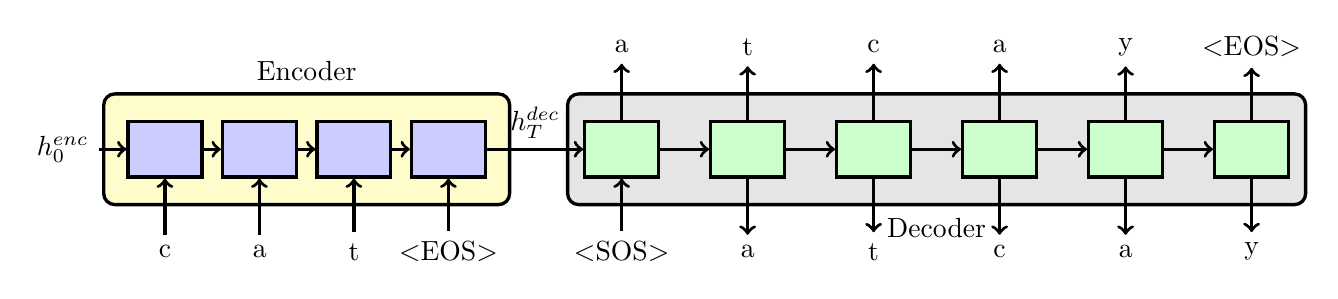
\begin{tikzpicture}[very thick]
        \node[block1, fill=yellow!20] (a) {};
        \node[block1, fill=gray!20, right of=a, text width=26em, node distance=8cm] (b) {};

        \node[above of=a] (z1) {Encoder};
        \node[below of=b] (z2) {Decoder};

        \node[block2, left of=a, node distance=1.8cm] (c1) {};
        \node[block2, left of=a, node distance=0.6cm] (c2) {};
        \node[block2, right of=a, node distance=0.6cm] (c3) {};
        \node[block2, right of=a, node distance=1.8cm] (c4) {};

        \node[block3, left of=b, node distance=4.0cm] (d1) {};
        \node[block3, left of=b, node distance=2.4cm] (d2) {};
        \node[block3, left of=b, node distance=0.8cm] (d3) {};
        \node[block3, right of=b, node distance=0.8cm] (d4) {};
        \node[block3, right of=b, node distance=2.4cm] (d5) {};
        \node[block3, right of=b, node distance=4.0cm] (d6) {};

        \node[below of=c1, node distance=1.3cm] (e1) {c};
        \node[below of=c2, node distance=1.3cm] (e2) {a};
        \node[below of=c3, node distance=1.3cm] (e3) {t};
        \node[below of=c4, node distance=1.3cm] (e4) {$<$EOS$>$};
        \node[left of=c1, node distance=1.3cm] (e5) {$h_0^{enc}$};
        \draw[->] (e1) -- (c1);
        \draw[->] (e2) -- (c2);
        \draw[->] (e3) -- (c3);
        \draw[->] (e4) -- (c4);
        \draw[->] (e5) -- (c1);
        \draw[->] (c1) -- (c2);
        \draw[->] (c2) -- (c3);
        \draw[->] (c3) -- (c4);

        \node[below of=d1, node distance=1.3cm] (f1) {$<$SOS$>$};
        \node[above of=d1, node distance=1.3cm] (f2) {a};
        \node[above of=d2, node distance=1.3cm] (f3) {t};
        \node[above of=d3, node distance=1.3cm] (f4) {c};
        \node[above of=d4, node distance=1.3cm] (f5) {a};
        \node[above of=d5, node distance=1.3cm] (f6) {y};
        \node[above of=d6, node distance=1.3cm] (f7) {$<$EOS$>$};
        \node[below of=d2, node distance=1.3cm] (g3) {a};
        \node[below of=d3, node distance=1.3cm] (g4) {t};
        \node[below of=d4, node distance=1.3cm] (g5) {c};
        \node[below of=d5, node distance=1.3cm] (g6) {a};
        \node[below of=d6, node distance=1.3cm] (g7) {y};
        \draw[->] (f1) -- (d1);
        \draw[->] (c4) -- (d1) node[midway, above] {$h_T^{dec}$};
        \draw[->] (d1) -- (f2);
        \draw[->] (d2) -- (f3);
        \draw[->] (d3) -- (f4);
        \draw[->] (d4) -- (f5);
        \draw[->] (d5) -- (f6);
        \draw[->] (d6) -- (f7);
        \draw[->] (d1) -- (d2);
        \draw[->] (d2) -- (d3);
        \draw[->] (d3) -- (d4);
        \draw[->] (d4) -- (d5);
        \draw[->] (d5) -- (d6);
        \draw[->] (d2) -- (g3);
        \draw[->] (d3) -- (g4);
        \draw[->] (d4) -- (g5);
        \draw[->] (d5) -- (g6);
        \draw[->] (d6) -- (g7);
    \end{tikzpicture}
\end{document}